Das Ursprüngliche Ziel des Projektes war es, eine Drohne mittels Bewegungssteuerung zu Steuern.\\
Im Laufe des Projektes haben wir jedoch schnell festgestellt, dass dies in der kurzen Zeit und mit unserer begrenzten Erfahrung nicht möglich ist.
Um unser System trotzdem testen zu können, haben wir uns dazu entschieden ein kleines Demo-Game zu entwickeln.\\
Das Game wurde mit Unity3D erstellt, die Kommunikation mit dem Controller funktioniert über eine Serielle Schnittstelle und unserem eigenen Kleinen Protokoll.
Dabei war es uns wichtig, dass das die Kommunikation bidirektional erfolgen kann. Das heisst das der Benutzer mit dem Controller das Spiel steuern aber im Game den
Controller auch konfigurieren kann.\\

\begin{figure}[H]
  \begin{center}
    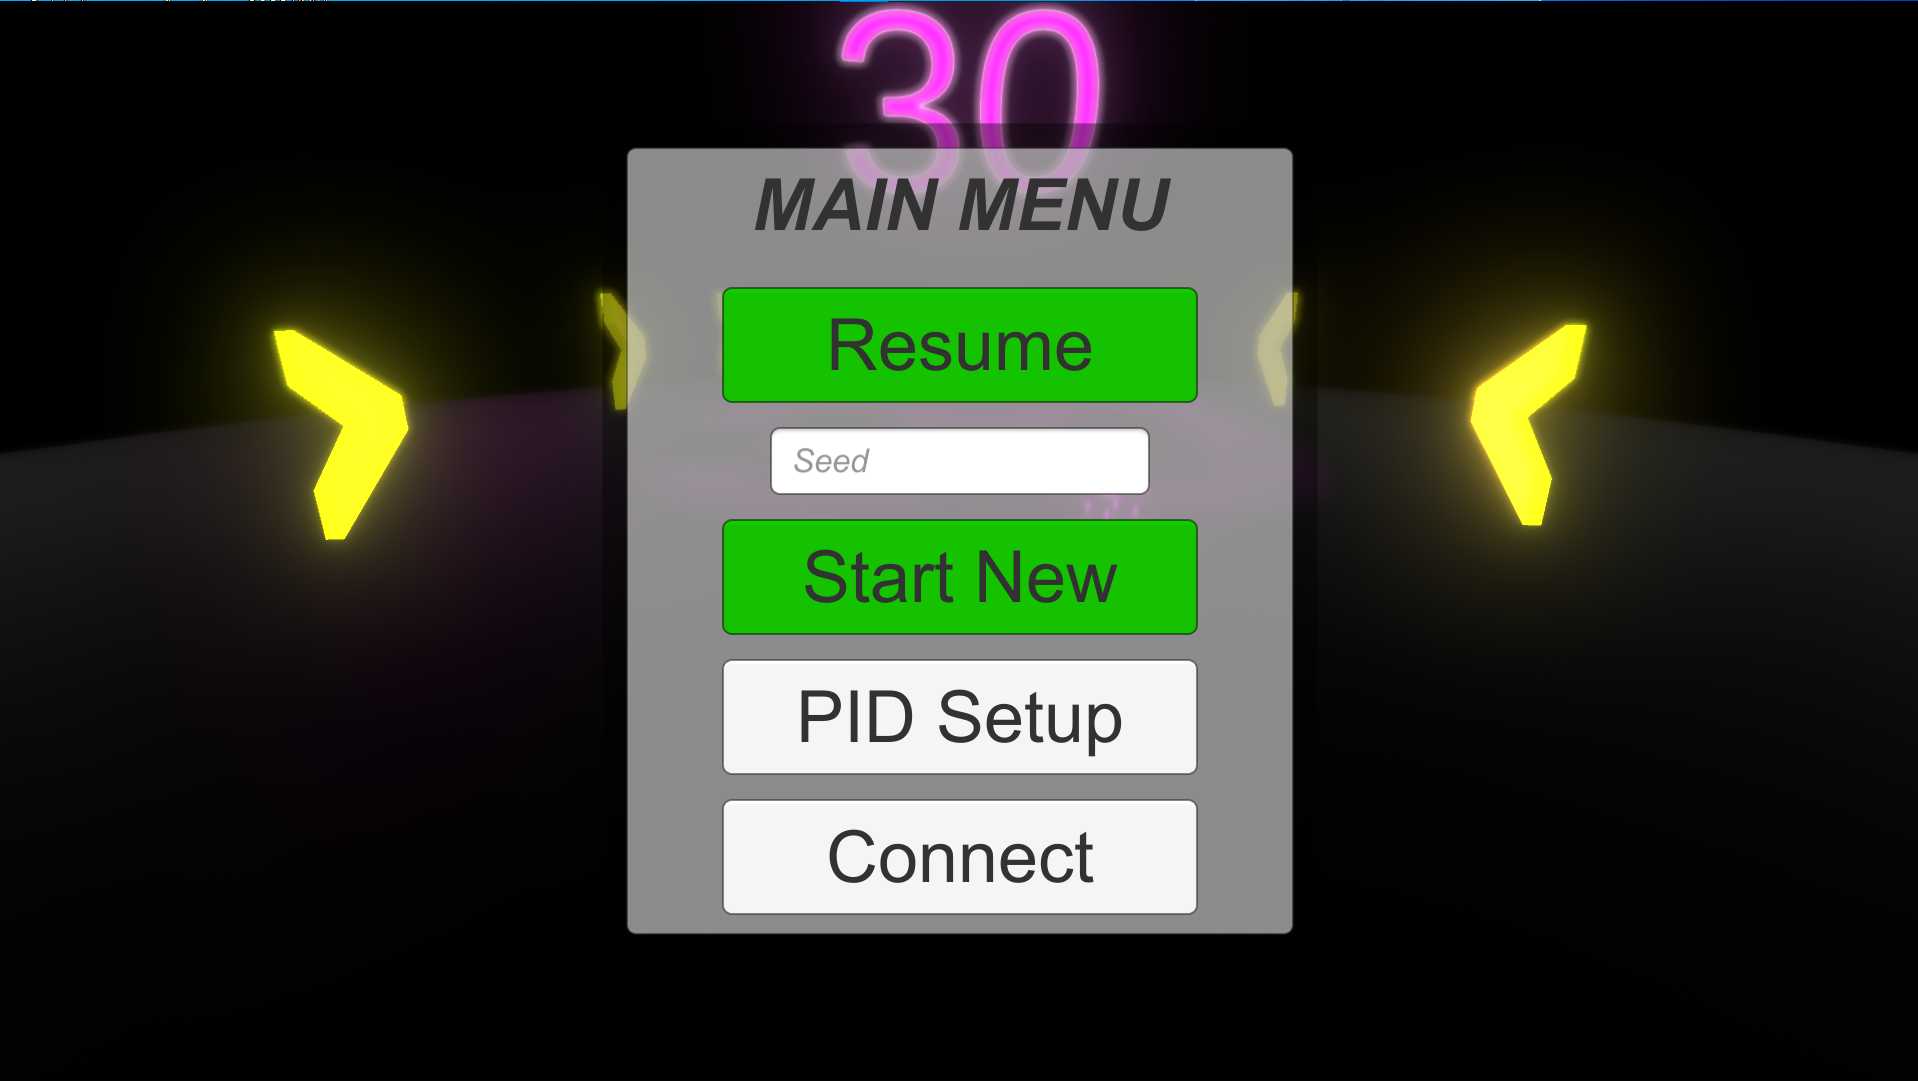
\includegraphics[width=0.6\linewidth]{content/images/menu1.png}
    \caption{Game Hauptmenu}
  \end{center}
\end{figure}

\begin{figure}[H]
  \begin{center}
    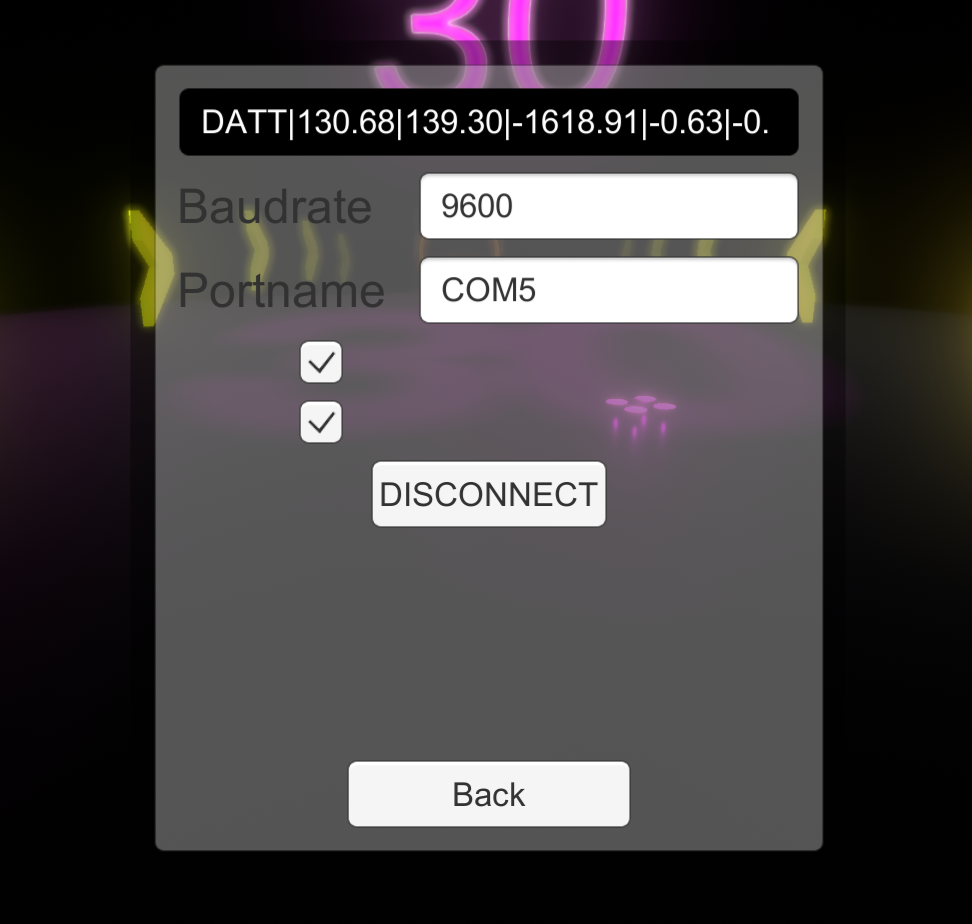
\includegraphics[width=0.6\linewidth]{content/images/connect.png}
    \caption{Verbindung herstellen}
  \end{center}
\end{figure}

\begin{figure}[H]
  \begin{center}
    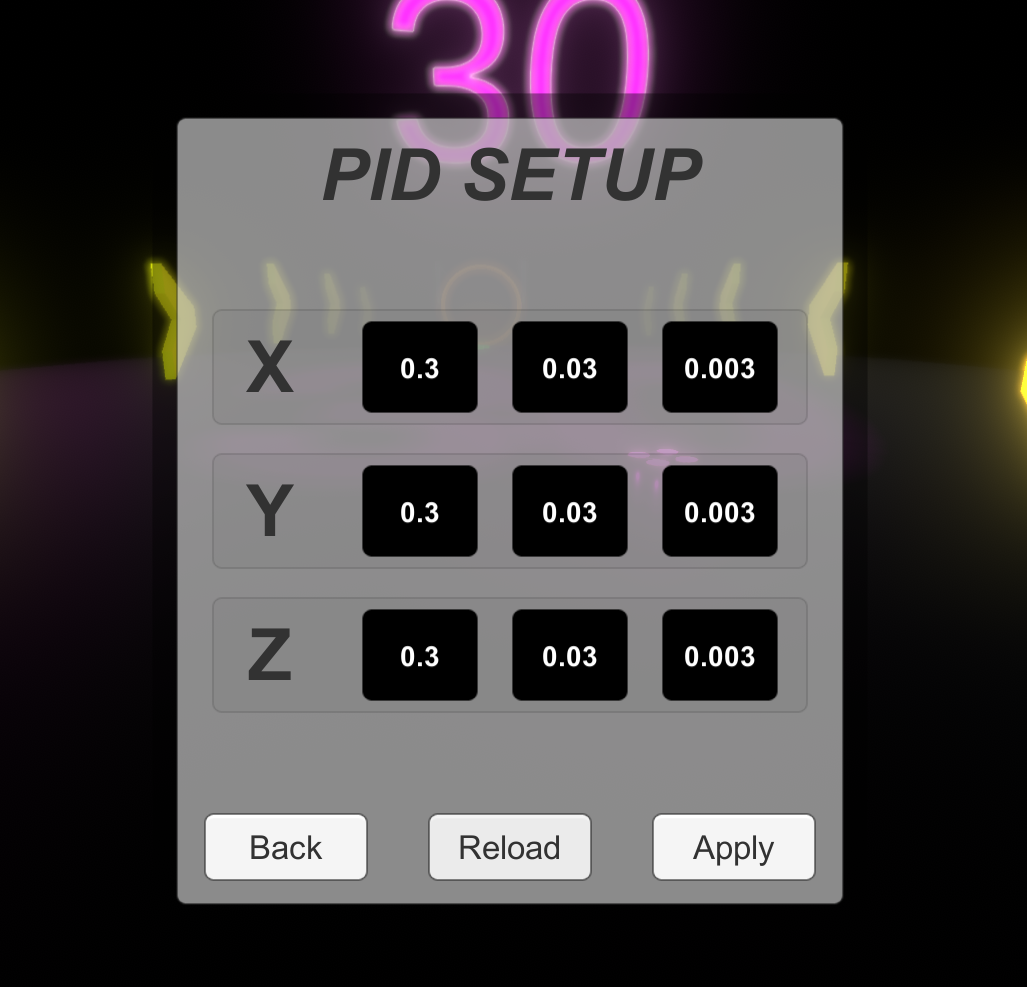
\includegraphics[width=0.6\linewidth]{content/images/PID.png}
    \caption{PID Einstellen}
  \end{center}
\end{figure}

\begin{figure}[H]
  \begin{center}
    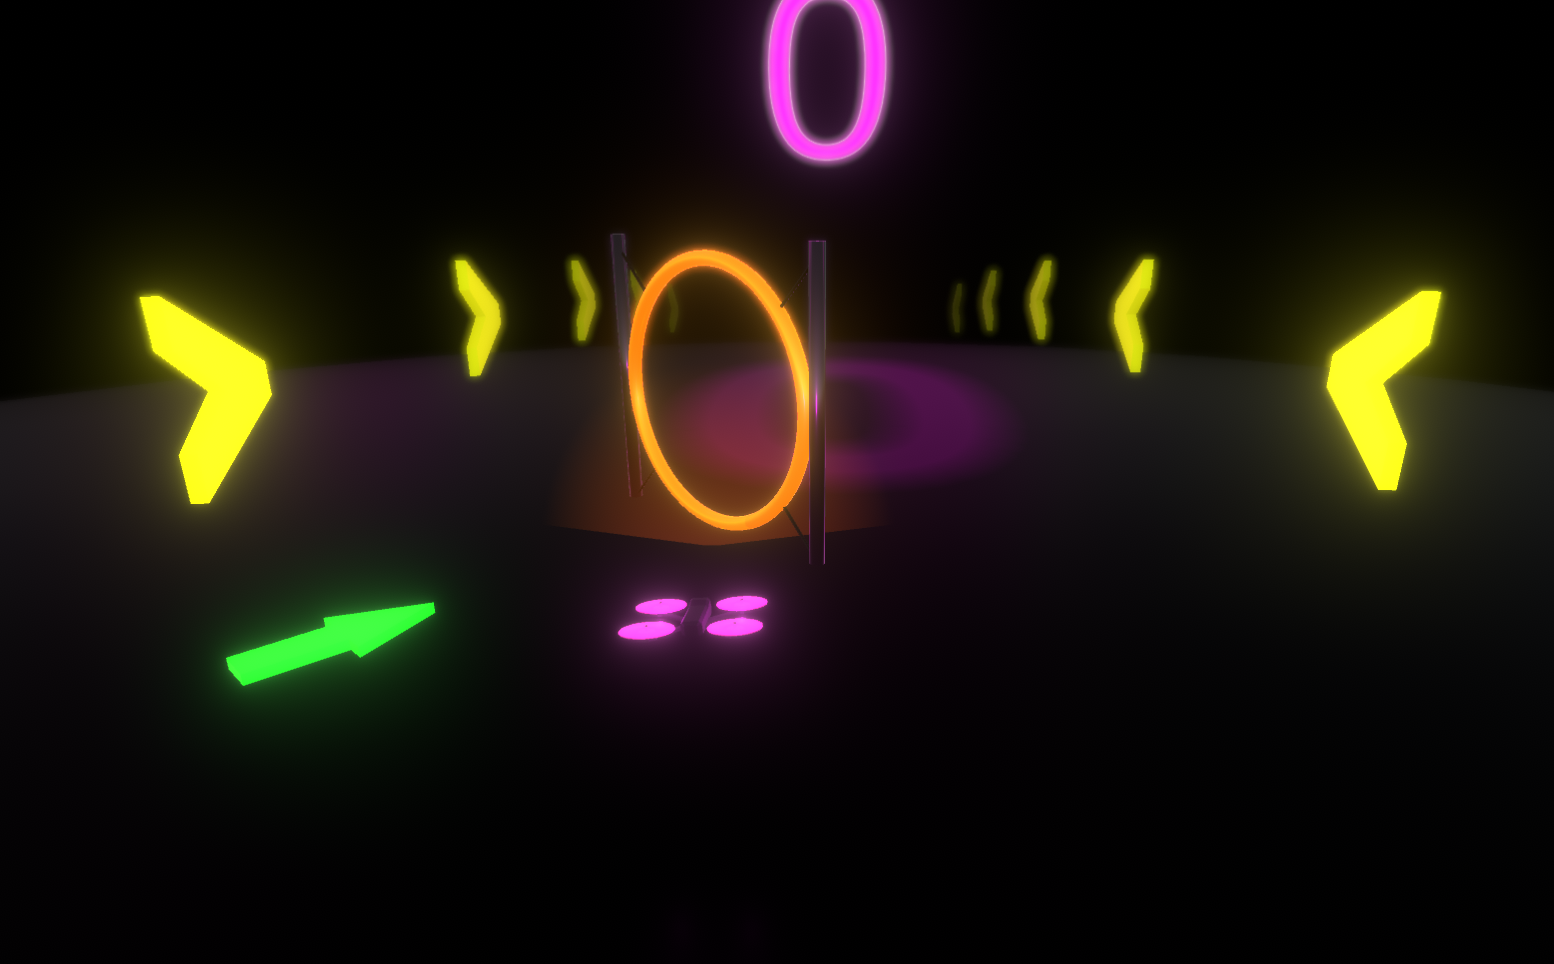
\includegraphics[width=0.6\linewidth]{content/images/game.png}
    \caption{In-Game Screenshot}
  \end{center}
\end{figure}